\section{Arjun Yuda Firwanda(1174008)}
\subsection{PYSHP Reader}
\begin{enumerate}
    \item Buatlah Script Python dan jelaskan berbaris
    \lstinputlisting[firstline=9, lastline=11]{src/1174008/3/soal1.py}
    \hfill\break
    \begin{figure}[H]
		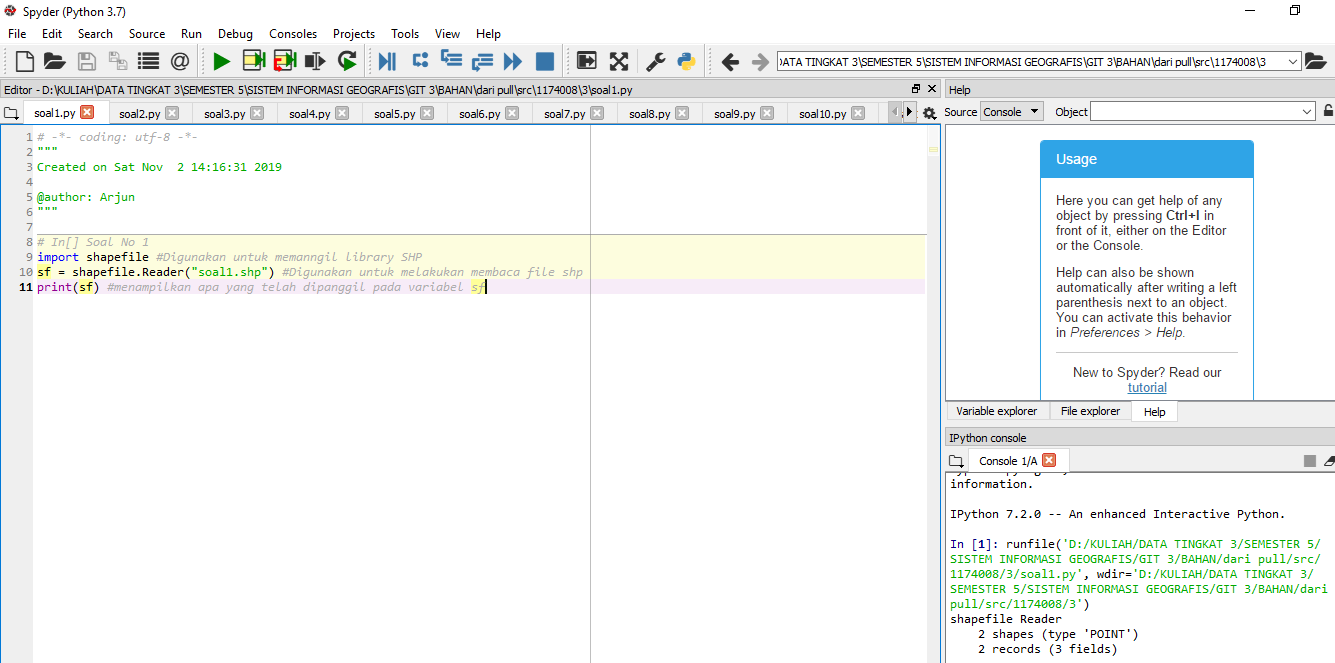
\includegraphics[width=4cm]{figures/1174008/3/soal1.PNG}
		\centering
		\caption{Hasil SHP Reader Soal 1}
    \end{figure}
    
    \item Buatlah Script Python dan jelaskan berbaris
    \lstinputlisting[firstline=9, lastline=12]{src/1174008/3/soal2.py}
    \hfill\break
    \begin{figure}[H]
		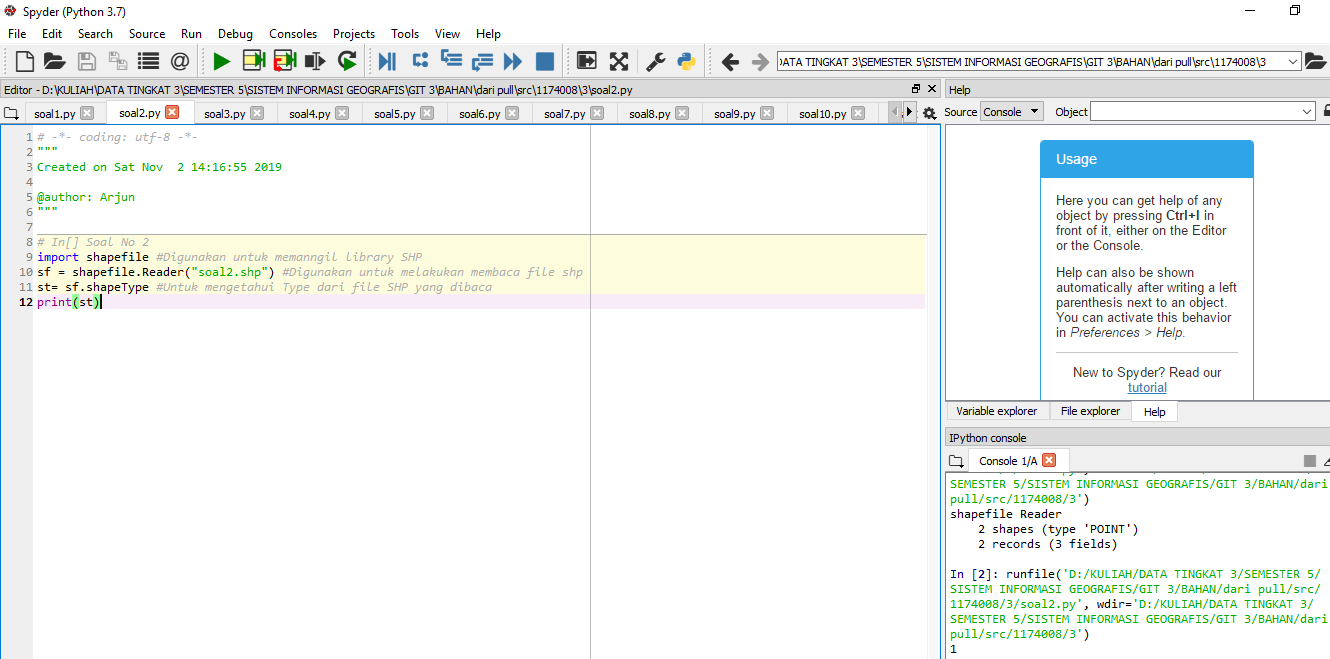
\includegraphics[width=4cm]{figures/1174008/3/soal2.PNG}
		\centering
		\caption{Hasil SHP Reader Soal 2}
    \end{figure}
    
    \item Buatlah Script Python dan jelaskan berbaris
    \lstinputlisting[firstline=9, lastline=12]{src/1174008/3/soal3.py}
    \hfill\break
    \begin{figure}[H]
		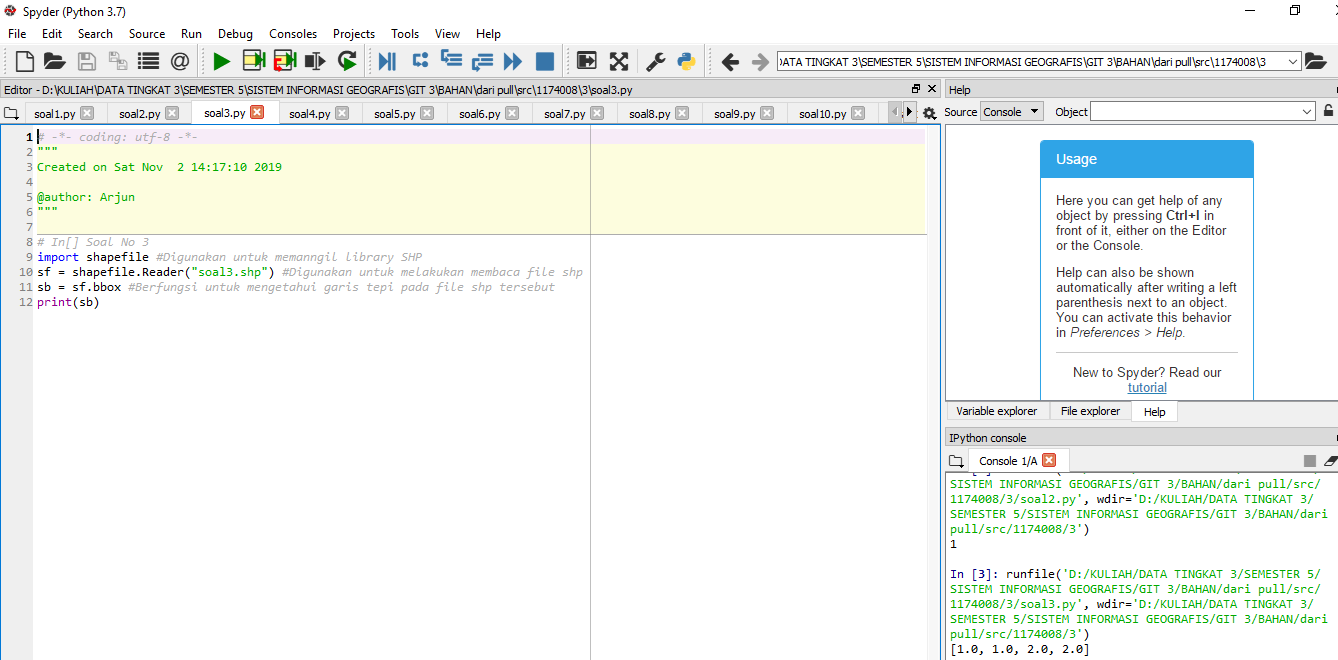
\includegraphics[width=4cm]{figures/1174008/3/soal3.PNG}
		\centering
		\caption{Hasil SHP Reader Soal 3}
    \end{figure}
    
    \item Buatlah Script Python dan jelaskan berbaris
    \lstinputlisting[firstline=9, lastline=12]{src/1174008/3/soal4.py}
    \hfill\break
    \begin{figure}[H]
		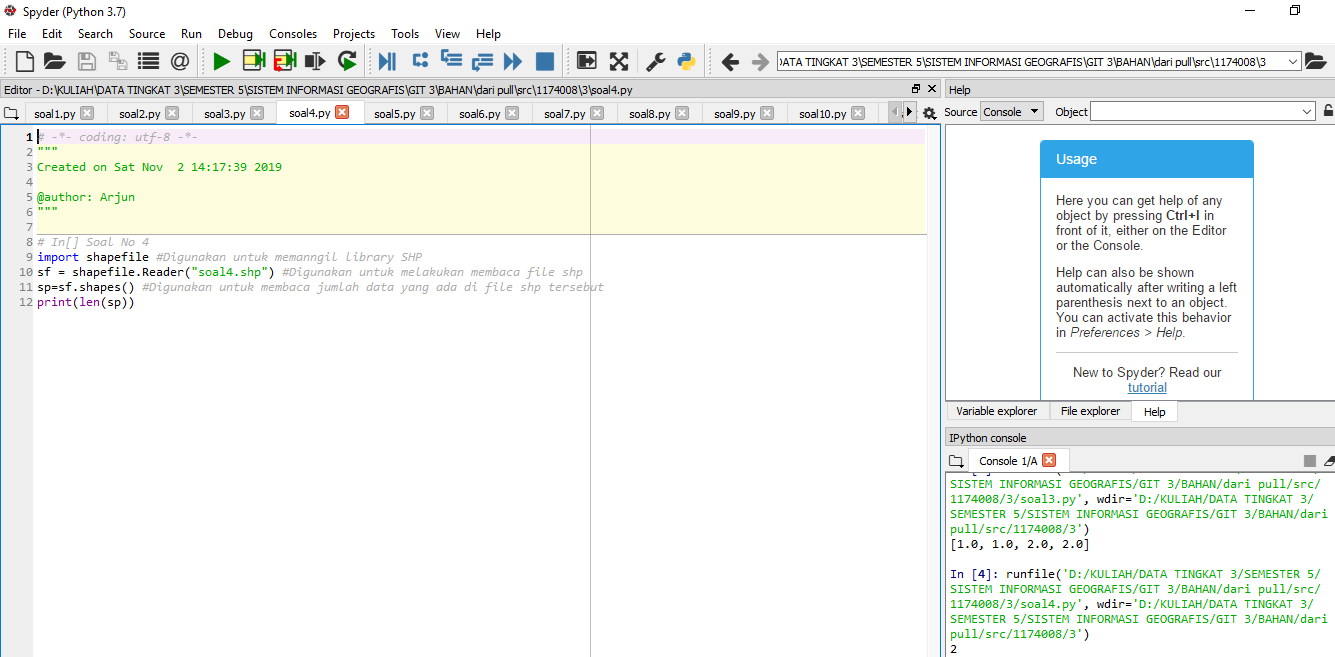
\includegraphics[width=4cm]{figures/1174008/3/soal4.PNG}
		\centering
		\caption{Hasil SHP Reader Soal 4}
    \end{figure}
    
    \item Buatlah Script Python dan jelaskan berbaris
    \lstinputlisting[firstline=9, lastline=13]{src/1174008/3/soal5.py}
    \hfill\break
    \begin{figure}[H]
		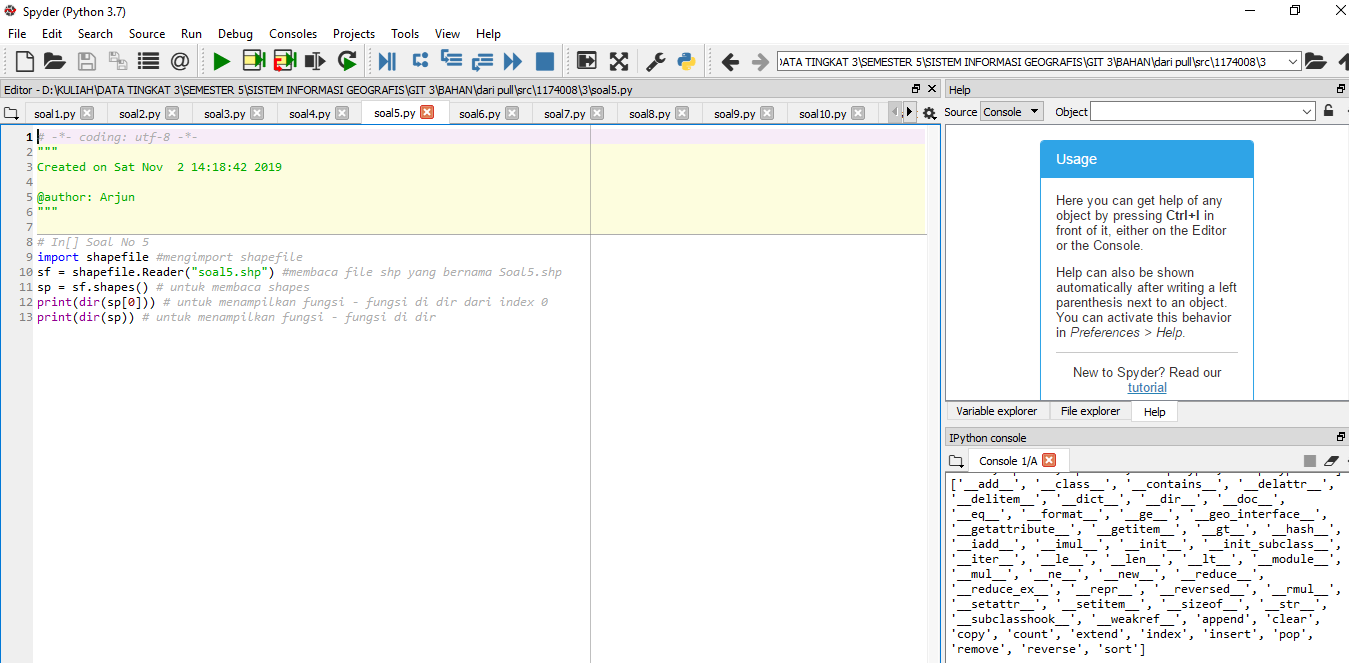
\includegraphics[width=4cm]{figures/1174008/3/soal5.PNG}
		\centering
		\caption{Hasil SHP Reader Soal 5}
    \end{figure}
  
    \item Buatlah Script Python dan jelaskan berbaris
    \lstinputlisting[firstline=9, lastline=13]{src/1174008/3/soal6.py}
    \hfill\break
    \begin{figure}[H]
		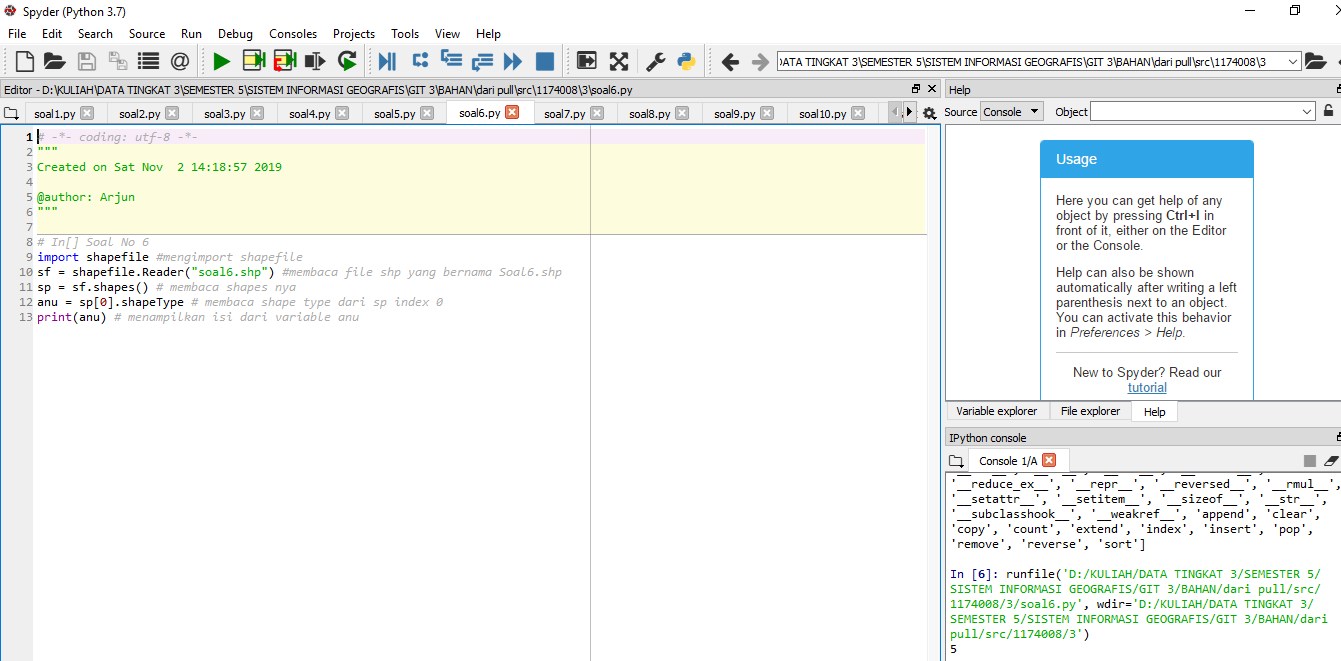
\includegraphics[width=4cm]{figures/1174008/3/soal6.PNG}
		\centering
		\caption{Hasil SHP Reader Soal 6}
    \end{figure}

    \item Buatlah Script Python dan jelaskan berbaris
    \lstinputlisting[firstline=9, lastline=13]{src/1174008/3/soal7.py}
    \hfill\break
    \begin{figure}[H]
		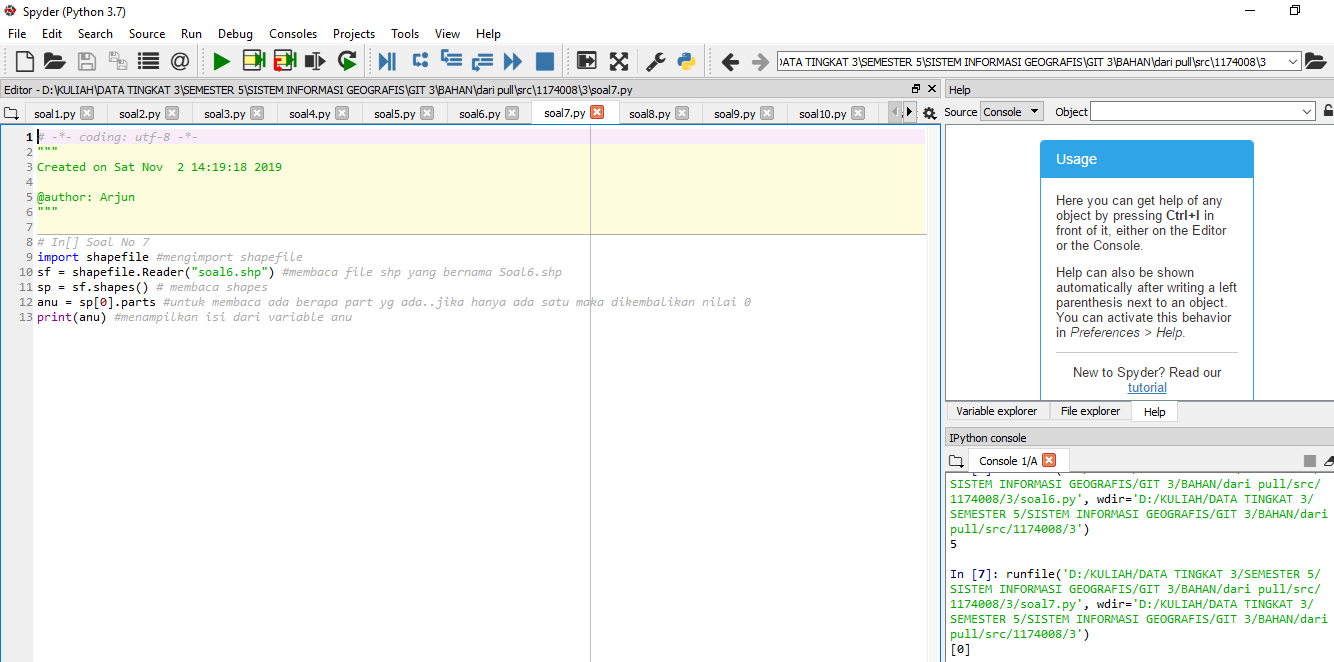
\includegraphics[width=4cm]{figures/1174008/3/soal7.PNG}
		\centering
		\caption{Hasil SHP Reader Soal 7}
    \end{figure}

    \item Buatlah Script Python dan jelaskan berbaris
    \lstinputlisting[firstline=9, lastline=13]{src/1174008/3/soal8.py}
    \hfill\break
    \begin{figure}[H]
		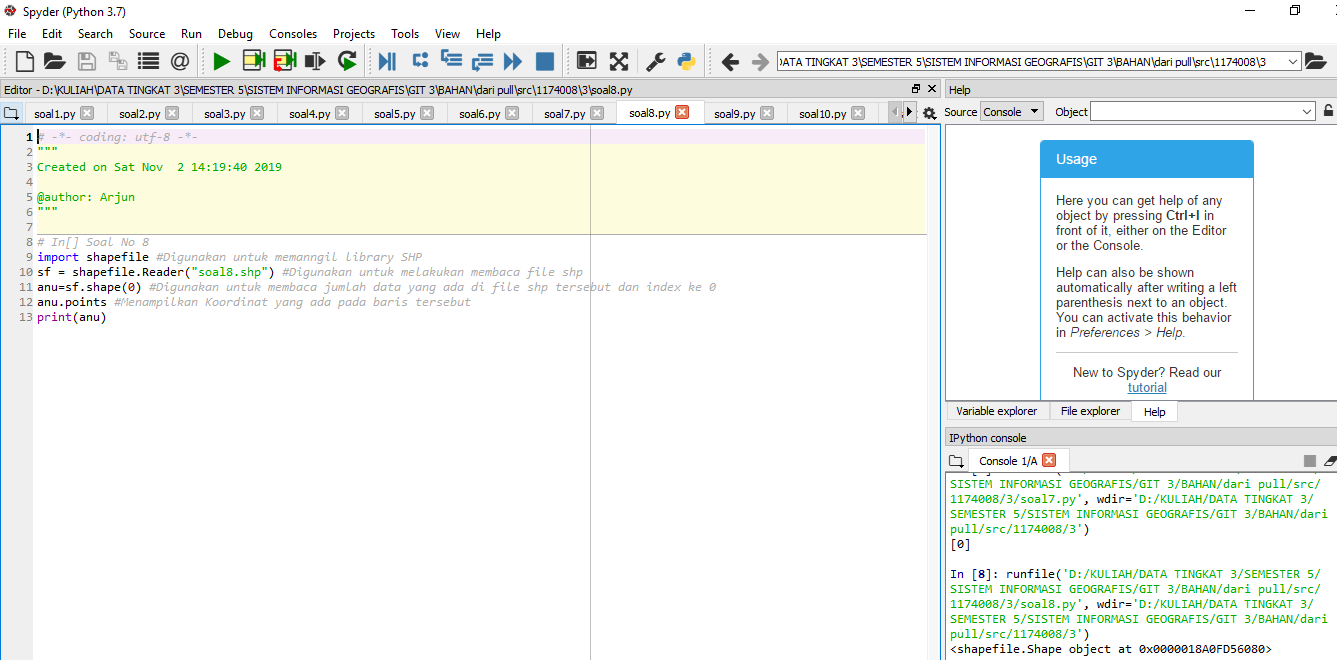
\includegraphics[width=4cm]{figures/1174008/3/soal8.PNG}
		\centering
		\caption{Hasil SHP Reader Soal 8}
    \end{figure}

    \item Buatlah Script Python dan jelaskan berbaris
    \lstinputlisting[firstline=9, lastline=12]{src/1174008/3/soal9.py}
    \hfill\break
    \begin{figure}[H]
		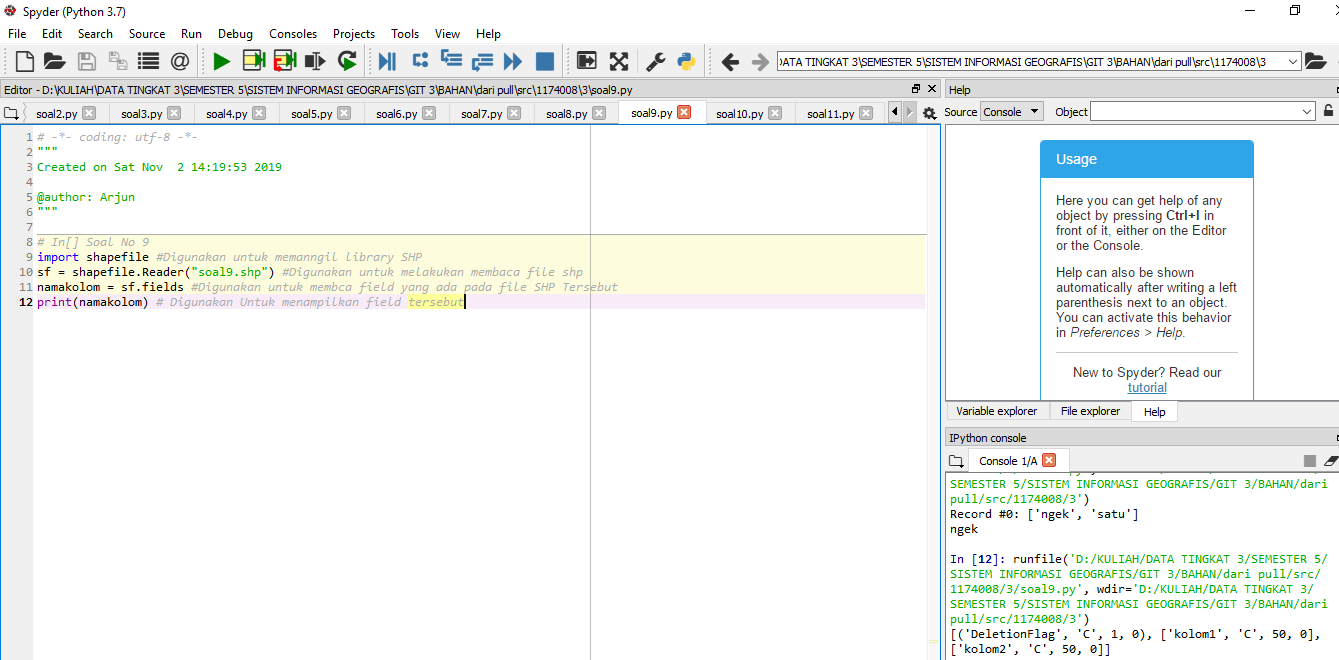
\includegraphics[width=4cm]{figures/1174008/3/soal9.PNG}
		\centering
		\caption{Hasil SHP Reader Soal 9}
    \end{figure}

    \item Buatlah Script Python dan jelaskan berbaris
    \lstinputlisting[firstline=9, lastline=12]{src/1174008/3/soal10.py}
    \hfill\break
    \begin{figure}[H]
		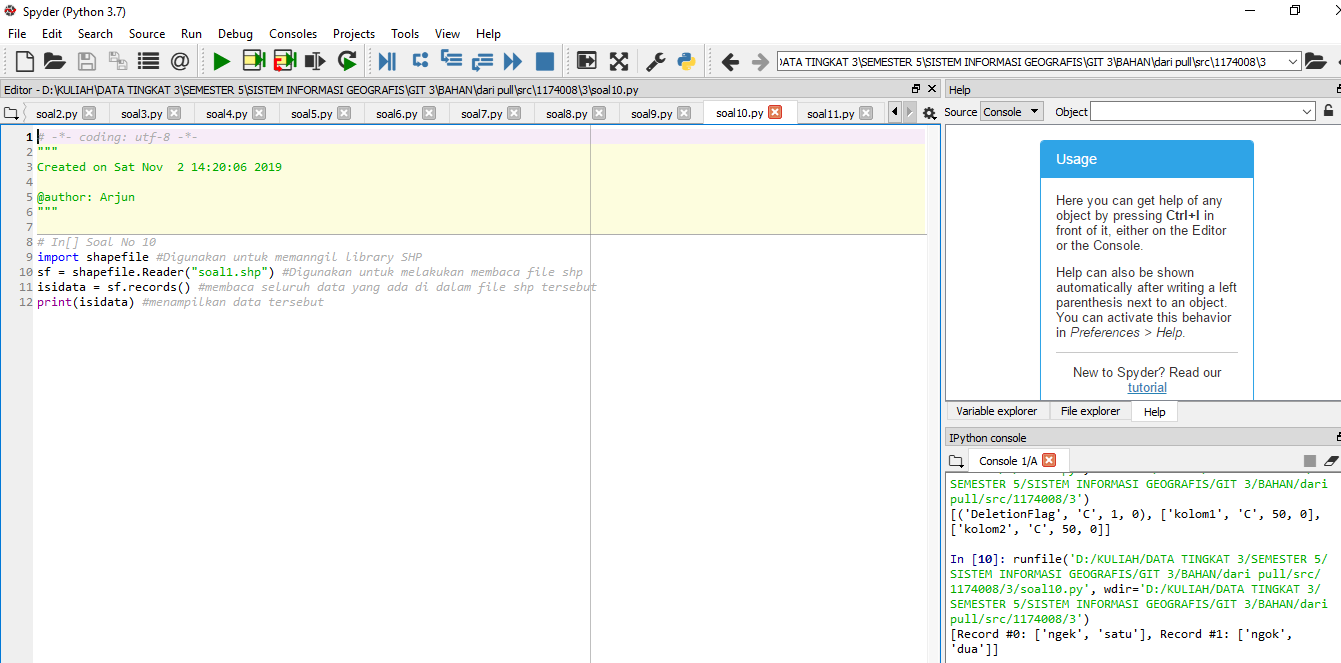
\includegraphics[width=4cm]{figures/1174008/3/soal10.PNG}
		\centering
		\caption{Hasil SHP Reader Soal 10}
    \end{figure}

    \item Buatlah Script Python dan jelaskan berbaris
    \item \lstinputlisting[firstline=9, lastline=13]{src/1174008/3/soal11.py}
    \hfill\break
    \begin{figure}[H]
		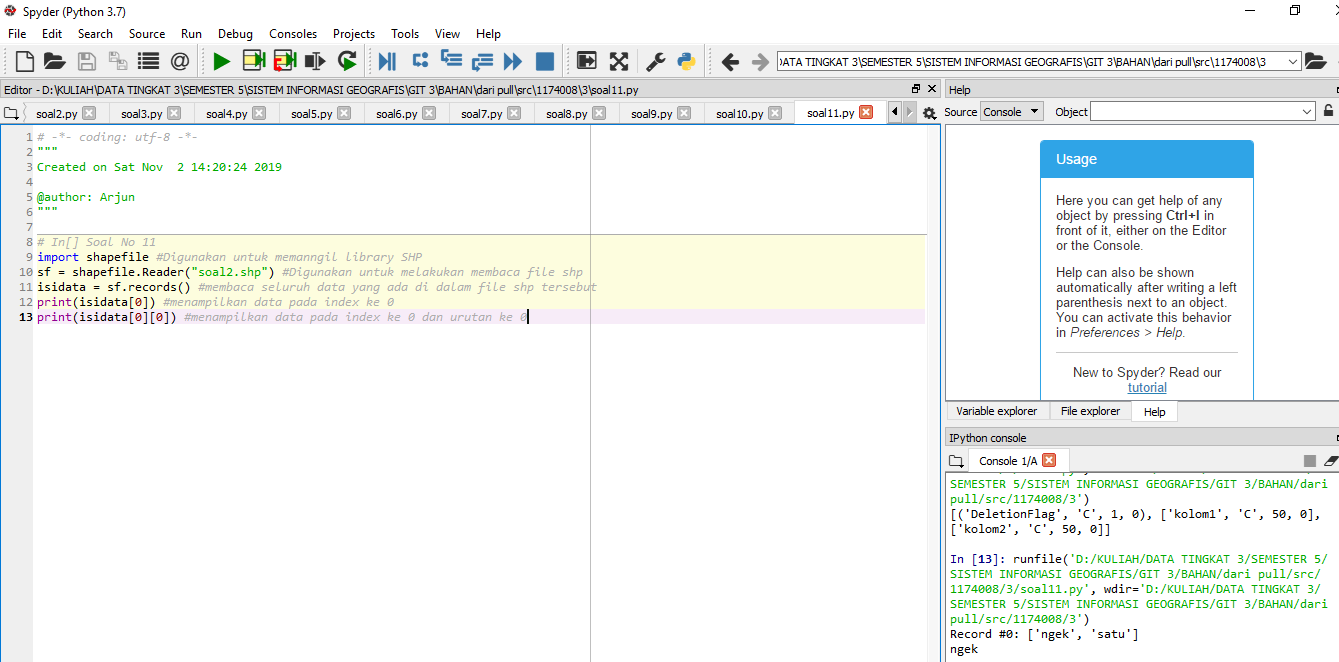
\includegraphics[width=4cm]{figures/1174008/3/soal11.PNG}
		\centering
		\caption{Hasil SHP Reader Soal 11}
    \end{figure}
\end{enumerate}
\subsection{Link Youtube}
\href{https://www.youtube.com/watch?v=0LQQ3pV4wUI&feature=youtu.be}{Video Youtube}